
%
% ---- Chapter layout ----
%
% 1) Introduction - 
% 2) 
% ------------------------



\chapter{Biogenic Isoprene emissions in Australia} % Chapter title
\label{BioIsop}
  
%----------------------------------------------------------------------------------------
% Section 1 -- INTRO 
%----------------------------------------------------------------------------------------
\section{Introduction}  
\label{BioIsop:intro}  
  
  % What we aim to do
  We estimate isoprene emissions in Australia using top-down estimates based on recalculated OMI HCHO measurements and modelled isoprene to HCHO yields.
  These estimates are compared to several campaigns (SPS1, SPS2, MUMBA, Daintree) and used as the new boundary conditions for GEOS-Chem.
  Sensitivity to soil moisture, (maybe) LAI, and satellite AMF calculation is examined and quantified for some scenarios.
  The effect of using these new top down isoprene emissions as the boundary conditions for GEOS-Chem is studied
  Wellness of fit between in-situ (at Wollongong) HCHO, satellite (OMI), and modelled (GEOS-Chem) HCHO is determined with and without updated emissions estimates.
  
  One of the most popular emissions inventories for biogenic isoprene, the Model of Emissions of Gases and Aerosols from Nature (MEGAN).
  Global atmospheric studies often use MEGAN along with a chemical transport model (CTM) to examine transport, deposition, and various chemical processes in the atmosphere.
  Emissions of Biogenic Volatile Organic Compounds (BVOCs) including isoprene are often the subject of studies as they are still relatively uncertain, as well as being drivers for imprtant oxidation and pollution events.
  
  (MEGAN) is poorly calibrated for Australian conditions, their emissions of isoprene (C$_5$H$_8$) may be overestimated, especially in the southeast.
  \cite{Muller2008} compared MEGAN against emissions calculated using top down estimates from the GOME2 satellite measurements of formaldehyde.
  \cite{Stavrakou2015} showed that this overestimate may be a factor of 2-3 in January.
  \cite{Sindelarova2014} show how 50\% of the isoprene emissions could be reduced by accounting for lower soil moisture.
  \cite{Emmerson2016} discuss the suitability of MEGAN's isoprene and monoterpene emission factors over southeast Australia, and suggest isoprene emissions are estimated 2-6 times too high.
  They also show that no blanket increase or decrease in emission factors is appropriate for the entire southeast of Australia.
  
  % Brief isoprene to hcho description
  In the remote troposphere HCHO production is dominated by methane oxidation, while in the continental boundary layer (CBL) production is largely due to NMVOCs (\cite{Abbot2003, Kefauver2014}).
  This suggests that HCHO enhancement over continents can be used to determine NMVOC emissions.
  In the CBL, HCHO enhancement is generally driven by short lived ($<1$~hr) precursors (most importantly isoprene).
  HCHO itself has a lifetime of a few hours (\cite{Kefauver2014}).
  Isoprene is emitted and enters the atmosphere in the gas phase, where it begins a complex series of reactions.
  Formaldehyde is produced with high yields in many of the isoprene reactions, which are discussed in more detail in Section \ref{LR:VOCs:IsopCascade}.
  HCHO measurements are often used as a check on how well isoprene reactions are simulated, as model output can then be compared against them \citep{Marvin2017}.
  
  
  
  % TODO: monoterpenes outline, here or elsewhere?
  Isoprene and monoterpene emissions are both very uncertain in Australia.
  Monoterpene oxidation by O$_3$, OH and NO$_3$ radicals may also form aerosols, with the reaction with ozone forming the most particles \citep{Kanakidou2005}.
  
  \subsection{Top-down emissions estimates}
    There are now a few methods of estimating isoprene emissions using satellite measurements of emission products, here I describe them and briefly compare the pros and cons of each.
    
    \subsubsection{Linear}
      \label{BioIsop:intro:top_down_linear}
      
      %TODO: Paul palmer outline of technique for top-down estimate
      This technique is the simplest, and is performed in this thesis.
      With the vertical columns of biogenic HCHO we can infer the local (grid space) isoprene emissions using effective molar formaldehyde yield (In other continents around 2-3, or 1 in low NO$_X$ conditions) \citep{Palmer2003,Marais2012,Bauwens2016}.
      If we assume there is fast HCHO yield, so that the effect of chemical transport is minimal, and that HCHO and isoprene are at steady states, then we can calculate local yield from our CTM.
      %This yield is derived from both HCHO and isoprene, such as was used by \citet{Millet2006} who produced a molar HCHO yield of 2.3 in north eastern USA.
      Yield is calculated from the modelled slope between isoprene emissions and HCHO total column within each gridbox over Australia, as performed in \cite{Palmer2003}, using modelled values between 1200-1400 LT which is around the overpass time of the OMI.
      This modelled yield is then used in conjunction with the recalculated OMI measurements in order to estimate isoprene emissions.
      To calculate emissions we use a reduced major axis (RMA) regression between modelled average values of the loss rates and total columns, an example is shown in figure TODO: figure with RMA of these over whatever time and space I end up using.
      
      % TODO: Pros and cons of PP top down method
      % Pros and cons:
    
    \subsubsection{Bayesian}
      Satellite based emissions estimates may allow us to improve the models without requiring lots of hard work on calibrating MEGAN to the large data sparse continent of Australia.
      Emissions of monoterpenes (C$_10$H$_16$, two units of isoprene) may also be underestimated in southeastern Australia, which could lead to the unique scenario of neither type of emission dominating VOC chemistry over the forests \citep{Emmerson2016}.
      
      % Top down emissions estimation methods:
      Another method of correcting isoprene emissions using observed HCHO total column involves a Bayesian inversion.
      \cite{Shim2005} work with GOME HCHO observations and GEOS-Chem, looking at areas with high signal to noise ratio (higher HCHO concentrations).
      They show that the model underestimates isoprene emissions and HCHO concentrations by 14-46\%, with the corrected VOC emissions reducing the model biases to 3-25\%.
      
      The Bayesian inversion is also used in \cite{Curci2010}, where a regional CTM (CHIMERE) simulates HCHO, which is compared against OMI observed HCHO and shown to be regionally biased.
      This bias is expected to be caused by errors in MEGANs isoprene emissions estimations.
      The CHIMERE model is used to derive yields of HCHO from the various local VOCs and these are then used in estimating local emissions.
      The model is run initially with emissions of BVOCs and reactive anthropogenic VOCs (RAVOCs) turned off in order to work out the background (b) values of these compounds.
      The Bayesian inversion is used to correct regionally biased biogenic isoprene emissions by optimising these parameters in order to simulate HCHO closest to the observed HCHO levels.
      \cite{Curci2010} uses CHIMERE as the forward model to determine the relationship between HCHO (y), isorene and reactive anthropogenic VOCs (\textbf{x}), using 
      \begin{equation}
      y=\mathbf{K}x + b + \epsilon
      \end{equation}
      where $\epsilon$ are the (assumed) independent errors in measurements.
      K is the Jacobian matrix determined from CHIMERE representing the sensitivity of y to the state variable x.
      This K matrix is used in conjunction with error covariance in x to determine the Maximum A Posteriori (MAP) solution to calculate the optimal estimate of x ($\hat{x}$).
  
  
  \subsection{Aims}
    
    %% AIMs paragraph
    Here we introduce how uncertain isoprene emissions are over Australia, and discuss literature which shows how the estimates may be too high.
    Section \ref{BioIsop:Data} describes the model, satellite, and campaign data we use to determine and analyse isoprene emissions.
    The OMI measurements used in this research are recalculated using an updated estimate of HCHO profiles and validated against Wollongong total column measurements.
    Section \ref{BioIsop:Methods} lays out how the isoprene emissions are estimated, and the results are examined in Section \ref{BioIsop:Results}
    
  
  
\section{Methods}
  \label{BioIsop:Methods}
  
  \subsection{Outline}
    % Method Briefly outlined here
    Here is an overview of the steps involved in my Thesis, which take satellite data and model output to estimate isoprene emissions.
    \begin{enumerate}
      \item 
        Download Aqua/Terra MODIS gridded fire counts (MOD14A1), smoke measurements (OMAERUVd), and Aura HCHO columns (OMHCHO).
        These products are discussed in more detail in Section \ref{Model:Datasets}.
      \item 
        Run GEOS-Chem with satellite overpass output averaged over 1200-1300~LT (matching Aura overpass time).
      \item 
        Recalculate OMHCHO vertical columns using GEOS-Chem to recreate the shape factors for each slant column. Also done with code from Paul Palmers group which includes recalculation of the scattering weights.
        The method to read the satellite data is given in Section \ref{Model:Datasets:OMHCHO}, while reprocessing the column AMFs is detailed in Section \ref{Model:omiRecalc}.
      \item 
        Mask HCHO columns which occur on days with non-zero (MODIS) fire counts over the prior 8 days, as is done in \cite{Marais2012}.
        More detail on this step can be found in \ref{Model:Filter:fire}
      \item 
        TODO: Filter gridsquares where OMI AAOD (OMAERUVd) is over some threshhold to be determined (ALSO TODO)
      \item 
        TODO: Filter NOx influenced grid squares.
      \item 
        Biogenic Yield calculated in each 2x2.5\degr grid square using daily averaged HCHO from biogenic only run of GEOS-Chem, linearly corellated with MEGAN isoprene emissions within those squares
      \item 
        TODO: Biogenic yield masked when smearing term is above a threshhold (TODO: determine)
      \item 
        Yield (actually regression slope between hcho and emissions) multiplied against recalculated OMI HCHO to provide top down isop emissions estimate
      \item 
        Compare against MEGAN, MUMBA, SPS, Daintree, Wollongong, and one set of airplane(?) measurements
    \end{enumerate}
  
  %TODO Full method outline to Jenny
  \subsection{}
  
  \subsection{Satellite inversion}
  \label{BioIsop:SatInv}
  
    % Lead in to satellite inversion
    Top-down estimates look at how much of a chemical is in the atmosphere and try to work out how much of its major precursors were emitted.
    This generally takes advantage of longer lived products which may reach a measurable equilibrium in the atmosphere.
    For isoprene this is done by looking at atmospheric HCHO enhancement, which can be largely attributed to isoprene emissions once transport and other factors are accounted for.
    Recently \cite{Stavrakou2015} used satellite HCHO measurements to constrain anthropogenic sources of isoprene and found good global agreement with the bottom up estimates, although some regions had sources differ by up to 25-40\%. 
    Their study used the RETRO 2000 database for anthropogenic emission aprioris except for Asia in 2008 where REASv2 was used. 
    Since 1997, when GOME first measured HCHO over Asia \citep{Thomas1998}, satellites have been able to provide a total column measurement of HCHO, one of the primary products of isoprene.
    
    Satellites recording reflected solar spectra use DOAS to measure various trace gases in the atmosphere, including formaldehyde. 
    While satellite measurements can only be used during daytime hours, HCHO lifetimes are sufficiently short that any night-time chemistry will not affect midday observations \citep{Wolfe2016}.
    Satellites can be used to measure the seasonal and interannual variability of HCHO over the globe.
    These records can be compared with modeled estimates of HCHO and used as a proxy to estimate isoprene emissions.
    This has been done in North America \citep{Palmer2003, Millet2006}, South America, Africa, China, Europe \citep{Dufour2009}, and recently globally \citep{FortemsCheiney2012, Bauwens2016}.
    Often these works use two forms of measurement such as satellite and aircraft data combined for validation (\cite{Marais2014}).
    There is less information available from satellite measurements at higher latitudes due to increased errors (\cite{DeSmedt2015}).
    
    Using HCHO to determine emissions of isoprene was initially performed by \cite{Palmer2001, Palmer2003}, who used in-situ summertime HCHO measurements over North America as model validation.
    Isoprene emissions fluxes were derived using the Global Ozone Monitoring Experiment (GOME) satellite instrument.
    Palmer's method improved biogenic isoprene emissions estimates (compared with in-situ measurements) over two available inventories: the U.S. EPA Biogenic Emissions Inventory System (BEIS2) and the Global Emissions Inventory Activity (GEIA).
    This showed an inversion technique which could be used to improve large scale emissions estimates without further expensive measurement campaigns.
    
    %TODO
    TODO: Read through this list of sources on the hcho to isop process : taken from Wolfe2015
    Such techniques have informed isoprene emission inventories in North America (Abbot et al., 2003; Millet et al., 2008 (\cite{Palmer2003,Millet2006,Palmer2006})), South America ((\cite{Barkley2013}), 2008), Europe (\cite{Curci2010,Dufour2009}), Africa (\cite{Marais2012}), Asia (Fu et al., 2007; Stavrakou et al., 2014), and globally (Fortems-Cheiney et al., 2012; (\cite{Shim2005}); Stavrakou et al., 2009).
    
    Initially studies assumed a simple linear steady-state relationship between HCHO and it's precursors (\cite{Palmer2003, Palmer2006, Millet2006}).
    This allowed a simple calculation of isoprene using the measured HCHO, with estimated reaction rates and yields.
    The methodology for calculating VOCs from HCHO is laid out in \cite{Palmer2003}, and takes into account the expected lifetime and reaction rates of the precursor VOCs and HCHO.
    Assuming HCHO is produced quickly from short-lived intermediates, and the column is at steady state:
    \begin{eqnarray*}
      VOC_i \overset{k_i}{\rightarrow} Y_i HCHO
    \end{eqnarray*}
    Where $Y_i$ is HCHO yield per C atom (a measure of how much HCHO will form per gram of C from a VOC within a system), and $k_i$ is the reaction rate.
    Then assuming a steady state of atmospheric HCHO ($\Omega$ molecules $cm^{-2}$) produced by oxidation of VOCs (VOC$_i$) and no horizontal transport:
    \begin{eqnarray*}
      \Omega = \frac{1}{k_{HCHO}} \sum_{i} Y_i E_i
    \end{eqnarray*}
    Where i indexes a chemical species, $k_{HCHO}$ is the HCHO loss rate due to OH and photolysis, Y$_i$ is the molar HCHO yield from oxidation of i, and $E_i$ is emission fluxes ( C atoms $cm^{-2}s^{-1}$).
    
    Estimates of Y$_i$ can be attained from a model as shown in \cite{Millet2006}.
    This involves a reduced major axis (RMA) correlation calculation between modelled HCHO and isoprene columns, multiplied by their loss rates (to photolysis and oxidation) (as a normalising factor).  
    In high NOx environments where HCHO has a lifetime on the order of 30 minutes, it can be used to map isoprene emissions with spatial resolution from 10-100 kms.
    Horizontal transport 'smears' the HCHO signal so that source location would need to be calculated using windspeeds and loss rates (\cite{Palmer2001,Palmer2003}).
    Smearing is explicitly handled in these studies due to the importance of transport and NO$_X$ on forming robust and accurate estimates.
    Over Australia NO$_X$ levels are generally not high enough to ensure quick HCHO formation and we must take extra care that we can account for the transport or 'smearing' caused by slower HCHO formation, details on this process can be found in Section \ref{BioIsop:Methods:Smearing}.
    
    More recently, full inversions that better account for transport, source attribution, and chemical schemes have been implemented (\cite{FortemsCheiney2012}).
    TODO: full description of this better inversion technique going through FortemsCheiney2012.
    
    \cite{Kefauver2014} reviews remote sensing of BVOCs, which are on the rise, examining the last 20 years of data and analysis of the satellite products.
    Their review encompasses the latest reports up to 2014.
    The modelled isoprene and BVOC emissions from MEGAN \citep{Guenther2000} of 500 and 1150~Tga$^{-1}$ respectively are still the global go to estimates.
    Their review reinforces the message that NMVOCs affect the oxidative capacity of the atmosphere and are largely driven by and sensitive to vegetation.
    The tropospheric affects from NMVOCs on the hydroxyl radical (OH), ozone (O$_3$), SOAs, and methane longevity, all interconnect to form a very complex system which still suffers from relatively large uncertainties in both measurement and chemistry mechanisms.
    One focus of \cite{Kefauver2014} is HCHO, which is the dominant product of most BVOCs which is measurable by remote sensing.
    The main datasets of HCHO are from four satellite instruments: GOME on ERS-2, SCIAMACHY on ENVI-SAT, OMI on EOS AURA, and GOME2 on MetOp-A.
    These satellites have slightly different spectral and spatial resolutions, as well as using varied processes to estimate HCHO from detected radiances.
    This can lead to different estimates between instruments or methodologies as described in \cite{Lorent2017}, which means validation and comparison is more important when using these remotely sensed data.
    
    Total HCHO is measured by satellite over the entire world, however the technique is not perfect and suffers from uncertainties and interferences.
    Satellite based chemical concentrations rely on ground-based measurements and modelled data for validation.
    They provide various readings with daily global coverage which is not otherwise feasable.
    
    Validation is important due to the various uncertainties in the satellite remote sensing process, with apriori assumptions having the greatest effect on structural uncertainty between measurements techniques \cite{Lorente2017}.
    \cite{Zhu2016} use SEAC$^4$RS aircraft HCHO measurements over the southeastern US as model validation, and show a bias in the assumed OMI shape factor that leads to a bias between satellite and SEAC$^4$RS measurements.
    \cite{Marais2014} compare OMI based isoprene emission estimates against relaxed eddy accumulation measurements from African field campaigns, as well as MEGAN and GEOS-5 inventories.
    \cite{Dufour2009} use HCHO from SCIAMACHY, and examine Europe using CHIMERE as the chemical model. 
    In their work they show that satellite measurements can reduce source emission uncertainty by a factor of two, where emissions are relatively large.
    
  \subsection{Calculation of Emissions}
    \label{BioIsop:Calculation}
   
    % FIRST: outline of what we do
    As is done in \citet{Palmer2003, Millet2006, Bauwens2016}, we assume that HCHO, and Isoprene columns are in a steady state, with no horizontal transport.
    We also assume that isoprene is the only compound enhancing the HCHO levels, which requires that we filter out influence from fires.
    Emissions of precursors are easy to calculate as long as we know the molar HCHO yields (Y$_i$) and effective chemical loss rates (k$_i$):
    \begin{equation}
    \Omega_{HCHO} = \frac{1}{k_{HCHO}}\Sigma_i k_i Y_i \Omega_i = \frac{1}{k_{HCHO}}\Sigma_i Y_i E_i
    \end{equation}
    This works if there is fast HCHO yield, so that the effect of chemical transport is minimal.
    The background HCHO is calculated using measurements in the remote pacific at the same time and latitude.
    Table \ref{BioIsop:Methods:tab_VOCAusYields} shows the average yield calculated for Australia. (TODO: this table and some notes)
    
    %% SLOPE Calculation
    In order to approximate the isoprene to HCHO yields over Australia, GEOS-Chem is run and the slope (S) between modelled tropospheric HCHO columns and emissions of isoprene within each grid box. 
    Figure (TODO: example grid box and regression plot.) shows the regression between emitted isoprene and tropospheric column HCHO, averaged between 1200-1300~LT each day.
    We can infer the local (grid space) isoprene emissions (E$_{isop}$) using effective formaldehyde yield from isoprene ($Y_{isop}$).
    \begin{equation} \label{BioIsop:Calculation:eqn_isop_yield}
    \Omega_{HCHO} = S \times E_{isop} + B
    \end{equation}
    Where \textit{B} is the background HCHO, and $S = Y_{isop}/k_{HCHO}$ is determined monthly as the regression between $\Omega_{HCHO}$ and E$_{isop}$ on daily saved outputs from GEOS-Chem over Australia using 2 by 2.5$^{\circ}$ horizontal resolution. 
    Modeled background emissions can be ignored here as they do not affect the slope calculation.
    Once we have calculated this slope, we use the same formula (Eqn. \ref{BioIsop:Calculation:eqn_isop_yield}) to determine the isoprene emissions.
    By replacing $\Omega_{HCHO}$ and $B$ with OMI based values, $E_{isop}$ is the only unknown.
    
    %% NOTE: Satellite uncertainty bounds for slope calculation
    In several studies OMI satellite HCHO columns are scaled up by up to 40\% to match in-situ measurements TODO:citations.
    Since we don't have enough in-situ data to reasonably scale the satellite columns we instead re-run the calculation with them scaled up by 40\% and consider this as a possible bound on satellite uncertainty.
    Yield and estimated top-down emissions are therefore given an upper and lower bound on satellite based uncertainty through this method.
    
    %% BACKGROUND calculation(s)
    There are a couple of ways to determine the modelled background HCHO concentration, one of which involves running the model with isoprene emissions turned off, which allows us to see exactly how much the modelled isoprene emissions alter each vertical column of HCHO.
    This is effective since we have assumed variation in HCHO columns only depends on isoprene emissions, so our background term is theoretically identical to the emission free simulated HCHO.
    The other way involves looking at HCHO over the remote pacific at matching latitudes and times, which emulates how the background is determined for the measured HCHO.
    These modelled background HCHO concentrations are mostly used for comparison with other datasets.
    TODO: show how these two numbers compare! figure with time series of both backgrounds for Aus, SEAus, and remote ocean.
    
    The $B$ackground from OMI  is determined using the mean column HCHO measured over the remote pacific ocean (180-120$^{\circ}$W).
    TODO: Update the background term to do as follows: For this term we average each month of remote ocean measurements, as well as averaging longitudinally within 180-120$^{\circ}$W, and finally $B$ is estimated at each latitude using $\pm 10^{\circ}$.
    This is gives us a background which is appropriate for any latitude, and is shown in Figure TODO: figure with background region highlighted and a time series of background values.
    When calculating the $E_{isop}$ from our modeled slope with OMI HCHO and background, we end up with negative emissions wherever the OMI HCHO column is less than the OMI background (as $E_{isop} = \frac{\Omega_{HCHO} - B}{S}$).
    These are set to zero, which increases the average by around TODO: X\%.
    The measured background HCHO is the average concentration measured in the remote pacific at the same time.
    
    Figure \ref{BioIsop:Calculation:fig_E_isop_vs_hcho_model_sample} shows the modelled isoprene emissions and column HCHO concentrations along with the RMA regression line, sampled from grid boxes over Australia for January 2005.
    Some affects from the low emissions in grid boxes which are largely oceanic can be seen and are handled by TODO: handle these and document here.
    Due to the low horizontal resolution of GEOS-Chem (2 by 2.5$^{\circ}$, latitude by longitude), calculations from grid boxes on the coast which are largely oceanic need to be discarded as the change in HCHO is not dominated by emissions of isoprene, as is assumed for Eqn \ref{BioIsop:Calculation:eqn_isop_yield}.
    A nested version of GEOS-Chem allows a much better analysis of coastal regions, at 0.25 by 0.3125$^{\circ}$ resolution.
    \begin{figure}[!htbp]
      % Figure from GC_tests.py -> isop_hcho_RMA
      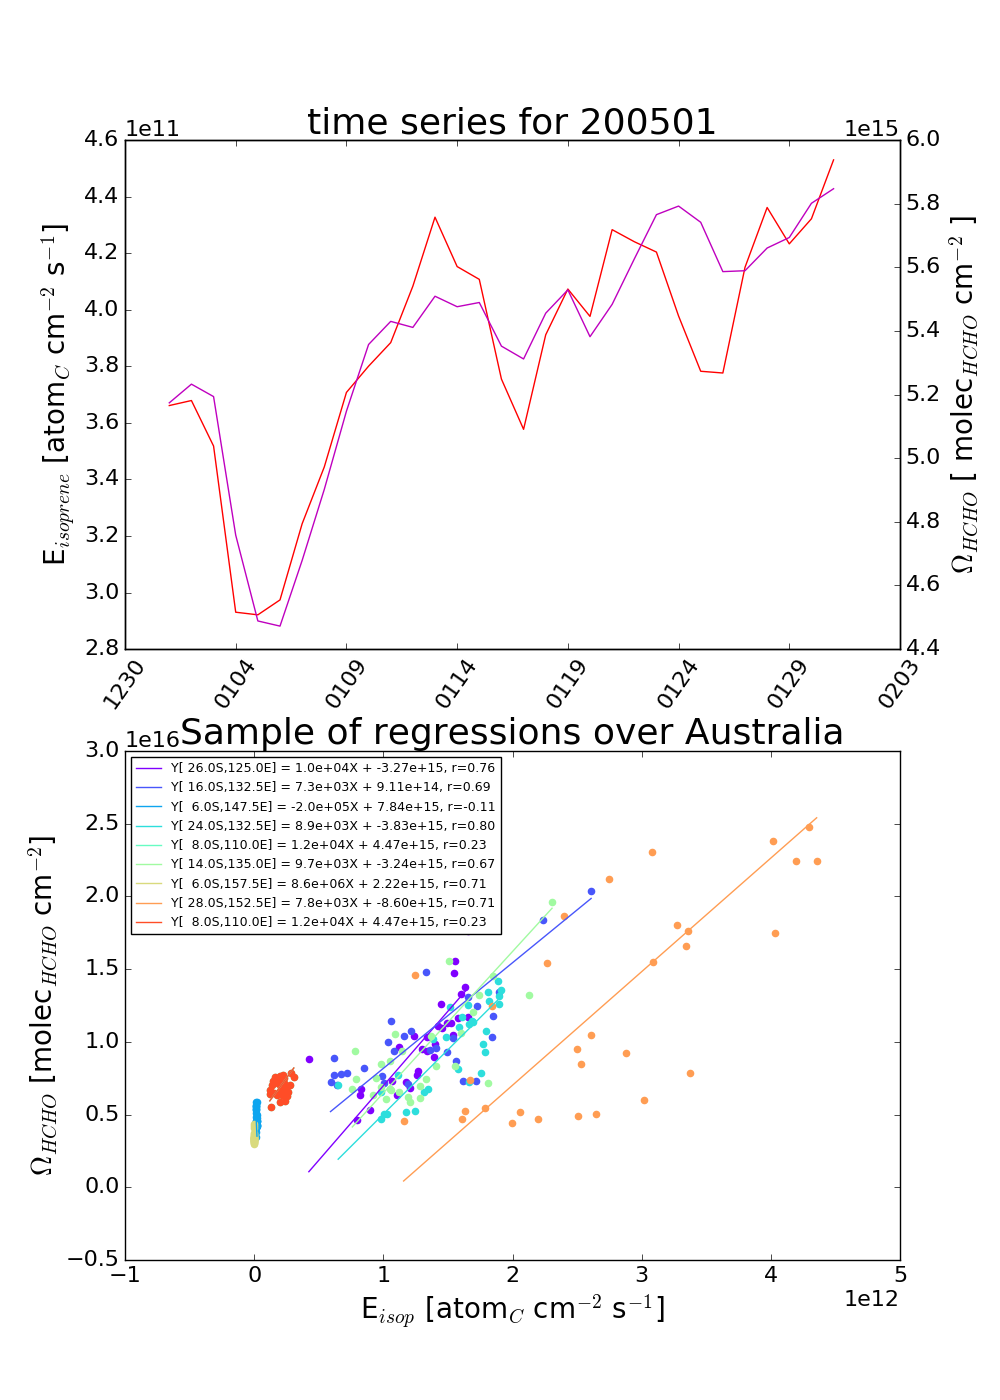
\includegraphics[width=\textwidth]{Figures/Isoprene/E_isop_vs_hcho_series_200501.png}
      \caption{%
        Top panel: isoprene emissions for January, 2005, shown in red, coplotted with tropospheric hcho columns, shown in magenta.
        Both series are daily averages over Australia.
        Bottom panel: (RMA) linear regressions from between emissions of isoprene and tropospheric hcho columns, sampled randomly from the 2$^{\circ}$ by 2.5$^{\circ}$ latitude longitude gridboxes over Australia for the month of January (2005).
      }
      \label{BioIsop:Calculation:fig_E_isop_vs_hcho_model_sample}
    \end{figure}
    
    %TODO: put this into results
    Using this modelled slope at 2$^{\circ}$ by 2.5$^{\circ}$ and applying it to equation \ref{BioIsop:Calculation:eqn_isop_yield} with B and $\Omega_{HCHO}$ calculated using OMI satellite measurements provides a new estimate of isoprene emissions.
    Figure \ref{BioIsop:Calculation:fig_E_isop_200501} shows the emissions calculated this way along with the Emissions output by GEOS-Chem averaged over January, 2005.
    \begin{figure}[!htbp]
      % Figure from Inversion.py -> check_against_MEGAN()
      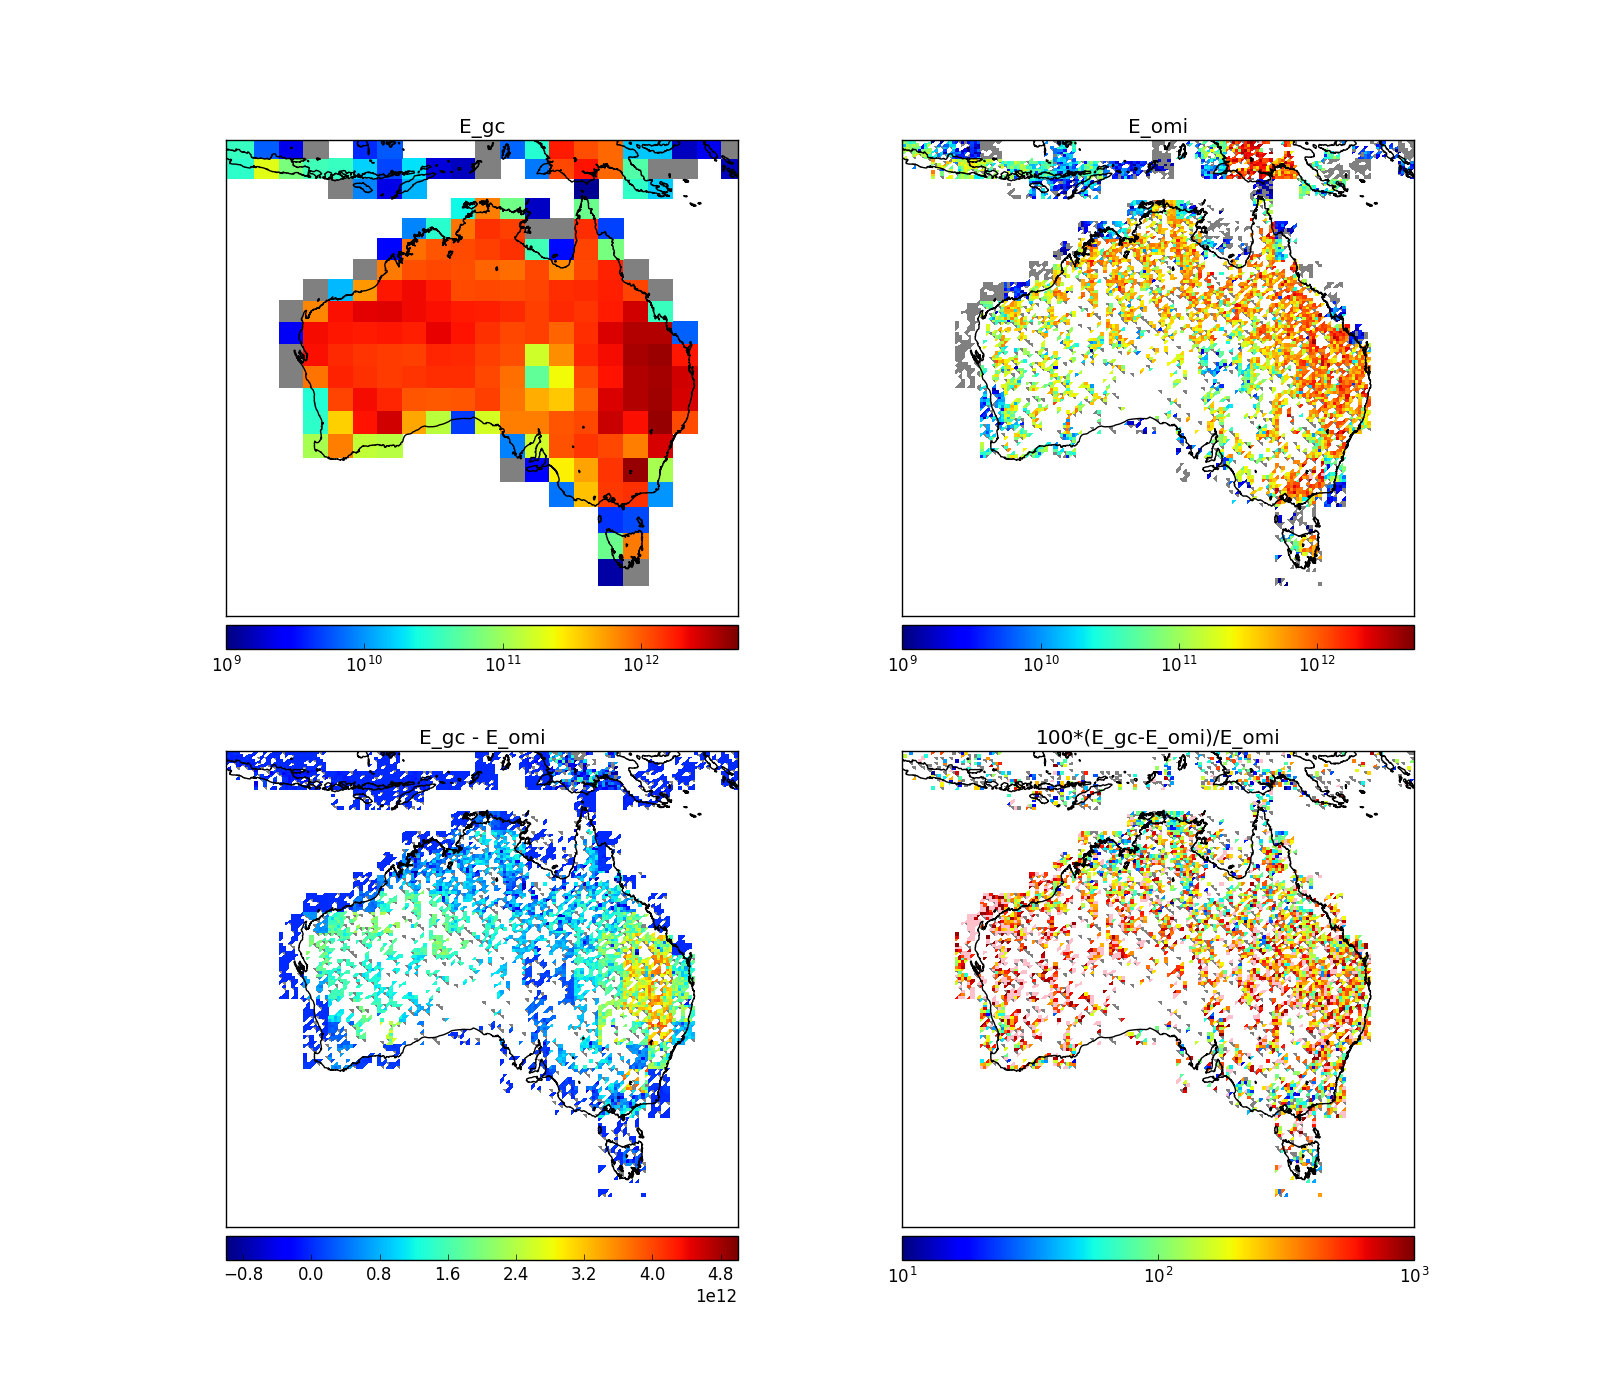
\includegraphics[width=\textwidth]{Figures/Isoprene/E_Comparison.png}
      \caption{%
        Top row is isoprene emissions for the month of January, in 2005, from GEOS-Chem and estimated from OMI respectively.
        Bottom row shows the absolute and relative differences between the two.
      }
      \label{BioIsop:Calculation:fig_E_isop_200501}
    \end{figure}
  
  \subsection{Emissions drivers}
    Calculated yields of HCHO can be classified using a box model which approximates specific environments, as described in Section \ref{BioIsop:CabbaMecca}.
    TODO: A table of different factors affecting emissions for three scenarios; urban, forest, shrublands is given in Table XX.
    The calculated yields for these scenarios is based on the CAABA/MECCA box model (described in Section \ref{BioIsop:CabbaMecca}) TODO: compare scenarios yields and show map of Australia with mapped closest scenario(one colour for each scenario, contourf).
    
  \subsection{HCHO Products and yield}
    \label{BioIsop:Methods:HCHOYield}
    Australian forests are strong emitters of both isoprene and monoterpenes, which go on to form various products including secondary organic aerosols, oxygenated VOCs (OVOCs), ozone, OH, and HO$_2$.
    This production occurs over several steps, yields are often classed into at least two categories.
    First generation yield refers to the amount of HCHO produced per unit isoprene consumed by initial oxidation, total yield (sometimes molar yield) refers to time dependent yield of HCHO over multiple oxidation stages \citep{Wolfe2016}.
    \citet{Wolfe2016} define prompt yield as the change in formaldehyde measurement per unit change in initial isoprene emissions.
    Some argue that isoprene emissions are overestimated, due to the fact that they are based on relatively few measurements of isoprene emission factors \citep{Winters2009, FortemsCheiney2012} TODO: read and cite paper mentioned in Fortems.
    Recently \cite{Emmerson2017} showed that MEGAN estimates 3-6 times too much isoprene emissions, and 4 times too little monoterpenes when compared against 4 (relatively small scale) measurement campaigns in southeastern Australia.
    
    Isoprene production of HCHO depends on several factors, importantly NO$_X$ levels have a direct effect on the fate of VOCs in the atmosphere.
    At higher NO mixing ratios (at least a few hundred pptv), organic peroxy radicals (RO$_2$) react mostly with NO. 
    At low NO (less than 10's of pptv), reaction with HO$_2$, other RO$_2$, and isomerization dominate the fate of RO$_2$.
    In low NO$_X$ environments, reported HCHO yields from isoprene are from XtoY\%, while in high NO$_X$ environments this value is XtoY\% TODO: these values from table.
    For monoterpenes the yields are around X, Y\% for low, high NO$_X$ respectively.
    Emissions and yields for various species including some terpenes can be seen in table \ref{BioIsop:Methods:tab_VOCAusYields}.
    \citet{Wolfe2016} determine that going from NO$_X = 0.1$ to $2.0$ ppbv triples the prompt yield of HCHO, from 0.3 to 0.9 ppbv ppbv$^{-1}$ due to isoprene, while the background HCHO doubles.
    They determine prompt yield as the change in HCHO per change in ISOP$_0$, using $[ISOP]_0=[ISOP]\exp(k_1[\mathrm{OH}]t)$; where $k_1$ is first order loss rate.
    This effectively relates HCHO abundance with isoprene emission strength.
    %TODO:and finish Wolfe2016 discussion paper for yields
    %TODO:go through atkinsonarey2003
    
    NO$_2$ measured by OMNO2d gives us a daily mid-day measurement which we can compare to output from GEOS-Chem to determine how well the model does at simulating NO$_2$.
    This is also done in \cite{Travis2016}, as a way to examine model bias in ozone (potentially due to NO$_2$ bias) over the USA.
    
    
    Looking at Australian emissions from running GEOS-Chem and using yields provided by XYZ (TODO other table), we see that Australia may be more or less likely to do something TODO: this comparison sentence would be good to tie up tables and be copied to conclusions.
    
    Conversions between HCHO per unit C yield and molar \% yield from species X given by the equation $ Y_{molar \%} = 100 \times C_X \times Y_{HCHO per unit C} $, where $C_X$ is how many Carbon are within species X (5 for isoprene, 10 for monoterpenes, etc...).
    For instance a 200\% molar yield of HCHO from isoprene implies 1 Mole of C$_5$H$_8$ becomes 2 Mole HCHO which is a 0.4 HCHO per unit C yield.
    
    TODO: Fill out this table
    \begin{table} \begin{threeparttable}
      \caption{HCHO yields from various species averaged over Australia during Summer.}
      \begin{tabular}{ | c  c  c  c  c | }
        \toprule
        \textbf{Species}   & \textbf{Emissions$^a$}& \textbf{Lifetime$^b$}& \textbf{HCHO Yield$^c$} & \textbf{HCHO production$^d$\%}
        \\                 & (Tg C per month)      &                      & (per C reacted)         &         \\
        \midrule
        Isoprene           & Y                     & n minutes            & 0.x                     & 10       \\
        $\alpha$-Pinene    & Y                     & n minutes            & 0.x                     & 10       \\
        $\beta$-Pinene     & Y                     & n minutes            & 0.x                     & 10       \\
        HCHO               & Y                     & n minutes            & 1.0                     & 10       \\
        \bottomrule
      \end{tabular}
      \begin{tablenotes} 
        \item a: Calculated using GEOS-Chem emissions over Australia in January 2005.
        \item b:  
        \item c: 
        \item d: Production determined by dividing emission*yield by the sum of all VOC emissions*yields. 
      \end{tablenotes}
      \label{BioIsop:Methods:tab_VOCAusYields}
    \end{threeparttable} \end{table}
    
    % yields from Atkinsen2003
    %isoprene
    %0.63 0.10 Tuazon and Atkinson (1990a)
    %0.57 0.06 Miyoshi et al. (1994)
    % a-pinene
    %0.23 0.09 Noziere et al. (1999a)
    %0.19 0.05 Orlando et al. (2000)
    % b-pinene
    %0.54 0.05 Hatakeyama et al. (1991)
    %0.45 0.08 Orlando et al. (2000)
    
    Yields table looking at literature provided yields of HCHO.
    % molar HCHO yield per unit carbon equal to HCHO molar percent yield(per carbon)? or some conversion?
    % TODO: ask steve about ppbv ppbv^-1 ??
    
    \begin{table} \begin{threeparttable}
      \caption{ HCHO yields from various species, and lifetime against oxidation by OH. }
      \begin{tabular}{  l  l  l  l  l  }
        \toprule
        Species    & HCHO Yield    & Life vs OH   & NO$_X$ background & Source   \\
                   & (molar \% )   &              &                   &          \\
        \midrule 
        Isoprene	& 315$\pm$50      &            & High          & a        \\ 
                  & 285$\pm$30      &            & High          & a        \\ 
                  & 225             & 35 min     & High          & b        \\ % Done
                  & 150             &            & Low           & b        \\ % Done
                  & 150             &            & Low           & d        \\
                  & 450             &            & High          & d        \\
                  & 235             &            & 1~ppbv        & e        \\
                  & 150             &            & 0.1~ppbv      & e        \\
        $\alpha$-Pinene & 28$\pm$3        &        & Low                & c        \\ 
                        & X$\pm$3         &        & X                  & d        \\ 
                        & 230$\pm$90      &        & High        & a        \\ 
                        & 190$\pm$50      &        & High        & a        \\ 
                        & 19              & 1 hour &              & b        \\ % Done
                        & 210             &        & 1~ppbv        & e        \\
                        & 70              &        & 0.1~ppbv      & e        \\
        $\beta$-Pinene  & 65$\pm$6        &        & Low           & c      \\ 
                        & X$\pm$3         &        & X             & d      \\ 
                        & 540$\pm$50      &        & High          & a     \\ 
                        & 450$\pm$80      &        & High          & a      \\ 
                        & 45              & 40 min &              & b      \\ % Done
        Methane 	      & 100             & 1 year  &             & b     \\ 
        Ethane          & 180             & 10 days &             & b     \\ 
        Propane         & 60              & 2 days  &             & b     \\ 
        Methylbutanol   & .13(per C)    & 1 hour  &             & b     \\ 
        HCHO            & 100             & 2 hour  &             & b     \\ 
        Acetone         & .67(per C)      & 10 days &             & b     \\ 
        Methanol        & 100             & 2 days  &             & b     \\ %Done
        \bottomrule
      \end{tabular}
      \begin{tablenotes} % \item makes new lines
        \item a \citet{AtkinsonArey2003}: Table 2, Yield from Isoprene reaction with OH, two values are from two referenced papers therein.
        \item b \citet{Palmer2003}: lifetimes assume [OH] is 1e15 mol cm$^{-3}$.
        \item c \citep{Lee2006}: Calculated through change in concentration of parent and product linear least squares regression.
        Estimates assume 20$^\circ$~C conditions.
        \item d \citet{Wolfe2016}: ``prompt yield'': change in HCHO per change in ISOP$_0$.
        $[ISOP]_0=[ISOP]\exp(k_1[\mathrm{OH}]t)$; where $k_1$ is first order loss rate.
        Effectively relates HCHO abundance with isoprene emission strength
        \item e \citet{Dufour2009}: One-day yields from oxidation modelled by CHIMERE, using MCM reference scheme.
        \item f Calculated using PTR-MS and iWAS on SENEX campaign data.
      \end{tablenotes}
      \label{BioIsop:Methods:tab_VOCLiteratureYields}
    \end{threeparttable} \end{table}
  
  
  \subsection{Accounting for smearing}
    \label{BioIsop:Methods:Smearing}
    
    Accounting for transport of the precursors is important, especially in low NO$_X$ conditions in which isoprene has a longer lifetime (days).
    When estimating emissions of isoprene using one of its products, it is often assumed that isoprene has a short lifetime, however when low NO$_X$ environments (which are prevalent in the Australian outback) this assumption can be wrong.
    Smearing (or spatial smearing) is a measure of how much formaldehyde (the product) was created from isoprene (the precursor) emissions in a different grid box.
    Smearing has been measured in order to account for this uncertainty in various works \citep{Martin2003,Palmer2003,Millet2006,Marais2012,Barkley2013,Zhu2014,Wolfe2016}, often implementing the method designed in \cite{Palmer2003}.
    
    Horizontal transport complicates estimation of precursor emissions, as the smearing length scale which increases beyond our gridbox size.
    The smearing length scale; the distance travelled downwind (L$_{d,i}$) by a precursor (i) before becoming HCHO can be estimated using:
    \begin{equation*}
      L_{d,i} = \frac{U}{k_i - k_{HCHO}} \ln{ \left( \frac{k_i}{k_{HCHO}} \right) }
    \end{equation*}
    where U is wind-speed.
    \citet{Palmer2003} further define a smearing length scale: L$_{s,i}$ as the distance downwind where a fraction (1 - $1/e$) of the precursor is completely transformed into HCHO.
    This equation uses the initial VOC column concentration ($[VOC]_0$) at the point of emission and mass balance equations as follows:
    \begin{equation}
    \frac{1}{k_{HCHO}-k_i} \left( k_{HCHO} \exp{ \left[ \frac{-k_i L_{s,i}}{U} \right]} -k_i \exp{ \left[ \frac{-k_{HCHO} L_{s,i}}{U} \right]} \right) = \frac{1}{e} 
    \end{equation}
    with limiting values L$_{s,i} \rightarrow U/k_i$ for $k_i << k_{HCHO}$, and L$_{s,i} \rightarrow U/k_{HCHO}$ for $k_{HCHO} << k_i$.  
    
    TODO: calculation of smearing
    Smearing sensitive grid boxes within the model can be detected by running the model with two times with only isoprene emissions changed.
    Similarly to smearing sensitivity calculations in \cite{Marais2012}, we run GEOS-Chem with isoprene emissions halved, then calculate $\hat{S} = \frac{\Delta \Omega_{HCHO}}{\Delta E_{Isop}} $, where $\Delta$ represents the monthly mean departure over 1300-1400LT from default run values.
    This allows us to determine which gridboxes are disproportionately affected by emissions from non-local sources.
    Consider halving the isoprene emitted globally and rerunning the model, you would expect HCHO enhancement (above background levels) to be halved in isoprene emitting grid-squares.
    If the local grid-square HCHO enhancement is reduced by much more than half (factoring yield) then you can infer sensitivity to non-local isoprene emissions.
    
    Smearing can be dependent on local or regional weather patterns, as greater wind speeds will reduce the time any emitted compound stays within the local grid box.
    As such smearing sensitivity is both spatially and temporally diverse, shown in figure TODO: is a picture of the smearing sensitivity over Australia.
    Large smearing values can be seen near many coastlines as the Emissions are very low, which makes transported isoprene relatively more important in these gridboxes.
    Once the smearing sensitive grid squares are filtered out, application of equation \ref{ch_isop:eqn:isop_yield} gives us an estimate of isoprene emissions across the nation.
    
    Most recently a \citet{Bauwens2016} undertook a similar process to what I am doing, although with slightly different focus, using the IMAGESv2 global CTM instead of GEOS-Chem.
    They calculate emissions which create the closest match between model and satellite vertical columns, and compare these postiori data with the apriori (satellite data) and independent data sets.
    (TODO: simple outline of what they did and how my focus is different, this paper will also need to be summarised in the LitReview)
    TODO: Plots of S hat showing worst smearing affected areas per season.
    
    
\section{Results}
  \label{BioIsop:Results}
  
  %TODO: Preliminary results shown at AGU - leading into other stuff
  
  \subsection{Emissions comparisons}
    
    Some global numbers (TODO: where do I throw these?)
    \citet{Guenther2012} Estimate global biogenic isoprene emissions at roughly 535\tgpyr, using MEGAN.
    \citet{Sindelarova2014} Estimate around 594\tgpyr using MEGAN with MACC, showing isoprene as 69.2\% of the total BVOC emissions, with monoterpenes at 10.9\tgpyr (10.9\%).
    They show 41\tgpyr decrease in Australia when introducing soil moisture parameterisation.
    
    When comparing the GEOS-Chem (which runs MEGAN) emissions to those calculated using our top-down inversion, we see a decrease over TODO: locations and seasons.
    TODO: table or figure showing summary of isoprene emissions changes over the whole of our time domain.
    
    Satellite measured HCHO has been found to be biased low in several studies \cite[eg.][]{Zhu2016,DeSmedt2015,Barkley2013}.
    These papers use in-situ data to scale up the satellite HCHO columns for their areas of interest, however Australia lacks sufficient HCHO measurements to do this.
    In these papers bias is seen as high as 40\%, which we use as our upper bound.
    Scaling up the satellite columns by 40\% gives us an upper bound on the uncertainty due to satellite bias.
    The 'Scaled Satellite' column refers to the calculations when using the 40\% scaled up OMI HCHO columns. %TODO: make table, add that column
    This can be considered as a boundary on satellite based HCHO column uncertainty.
    
    One set of data from the Daintree rainforest in Queensland exists (TODO: summary from P. Nelson).
    Although the data set lies outside our run times, as it was measured in TODO(runtime), we compare against the seasonal average of our GEOS-Chem output for the matching months (TODO: name the months).
    This is done for both GEOS-Chem output and our recalculated isoprene emissions.
    When compared against GEOS-Chem output we see TODO.
    When compared against recalculated emissions we see TODO.
    
    TODO: Figure showing campaign data against model and recalculated emissions over region for averaged months and eventually different resolutions.
    
    %As is done in \cite{Emmerson2016}, 
    We examine the affect of decreased isoprene emissions on the correlation between modelled and satellite based HCHO columns.
    Figure TODO: shows the regressions between GEOS-Chem tropospheric column amounts of HCHO and satellite columns for two runs of GEOS-Chem: a) using standard MEGAN emissions, b) using our updated emissions.
    
  \subsection{Emissions affect on GEOS-Chem}
    We interpolated or something (TODO) the emissions over Australia into the inventories used by GEOS-Chem which reduced the emissions by X\% per year (over Australia).
    The resulting simulation output shows that HCHO was reduced by X\%, although if we boost monoterpenes by X\% where the isoprene emissions were lowered then 
    
\section{Uncertainty}
\label{BioIsop:Uncertainty}

  There are several factors which need to be considered when looking at the uncertainty in emissions estimates.
  Things with their own inherent uncertainty include the modelled a-priori, modelled relationship between HCHO and isoprene, and satellite measurements. 
  Important factors which need to be analysed for confidence in results include the steady state assumptions, filtering techniques for fire and human influences, and the regression model for determining the isoprene to HCHO yield.
  
  Model uncertainty is difficult to accurately ascertain, generally an analysis of the model compared to in-situ measurements is performed, however there are few of these measurements over Australia.
  
  \subsection{Model Uncertainty}
    \label{Model:Uncertainty:Model}
    Uncertainty in modelled yield is estimated somehow (TODO:), and a upper and lower bound for the yield is determined using satellite scaling.
    Since OMI HCHO is scaled up by up to 40\% in several papers, we consider HCHO scaled by 1 and 1.4 to be boundaries for modelled yield calculations.
    These prior works use flight campaigns and in-situ data to verify HCHO columns in various locations (TODO: redo cite list from lit review).
    
    % uncertainty and sensitivity determined by CAABA/MECCA?
    
    % Link to satellite uncertainty
    
  % Subsection?
  \subsection{Satellite Uncertainty}
    \label{BioIsop:Uncertianty:Satellite}
    
    Uncertainty in satellite measurements is generally provided along with the data, although uncertainty introduced through AMF calculation needs to be determined to give a representation of the confidence in vertical column amounts.
    
    Provided with the OMI product is the measurement of uncertainty in each pixel, calculated by SAO from the backscattered solar radiation fit \citep{Abad2015,Abad2016}.
    BIRA use another method, and calculate the standard deviation of HCHO over the remote pacific ocean as the uncertainty \citep{DeSmedt2012, DeSmedt2015}.
    In the remote pacific, it can be assumed that HCHO variations are weak, with concentrations remaining steady in the short term ($\sim 1$ month).
    This means the standard deviation over this region can be used as a proxy for determination of the instrument error.
    
    There are three main sources of error in the resulting HCHO columns:
    \begin{description}
      \item[a] Fitting error from the OMI retrieval.
      \item[b] Uncertainty in AMF calculations.
      \item[c] Uncertainty of HCHO background.
    \end{description}
    
    a) is available in the OMI product and reduced through spatial and temporal averaging.
    Taking the eight day grided average with horizontal resolution of 0.25 by 0.3125 degrees (latitude by longitude) typically reduces uncertainty by a factor of 1.5 to 4.
    Another method for examining uncertainty of OMI is to analyse the standard deviation of the HCHO columns over the remote pacific.
    If we assume there is no HCHO variation from background levels over any 8-day period, then this method infers variations in the measuring instrument, and can be used as a metric for uncertainty as done in \citet{DeSmedt2012}.
    TODO: uncertainty calculation on remote pacific OMI.
    \cite{Millet2006, Palmer2006} both examine OMI HCHO columns over North America and determine overall uncertainty to be 40\%, with most of this coming from cloud interference.
    
    b) is determined through an analysis of GEOS-Chem output, validated against the total column of HCHO at Wollongong using FTIR measurements from the (TODO: Nicholas Jones roof HCHO citation here).
    \cite{Palmer2006} calculate the error in AMF through combining estimates of error in the UV albedo database ($\sim 8$\%), model error based on in-situ measurements, cloud error  ($20-30$\%) \citep{Martin2003}, and aerosol errors ($<20$\%), totalling AMF error of around $\sim 30$\%.
    It is worth noting here that independent error estimates are added in quadrature, which means total error equals the root of the sum of the independent errors each sqaured ($e_{Total}=\sqrt{\Sigma_i e_i^2}$).
    TODO:Paul palmer calculation and combination for overall Satellite VC uncertainty per pixel and gridded.
    TODO: Millet2008?
    
    c) is also determined through a study of GEOS-Chem output, in relation to in-situ measurements.
    TODO: calculate this uncertainty.
    Compare this error estimate with that of \citet{Curci2010}, where the error in b) and c) are respectively found to be 30\% and 15\% based on their analysis of CHIMERE.
    \cite{Millet2008} also examine this uncertainty and determine an overall uncertainty ($1\sigma$) of $25-27\%$ in HCHO vertical columns with calculated AMFs where cloud fraction $< 0.2$.
    
    
  
  
% Extras for potential paper output 
%  
%  \authorcontribution{}
%  \competinginterests{The authors declare that they have no conflict of interest.}%
%  \textit{Data availability.} All GEOS-Chem model output is available from the authors upon request.
%  %\disclaimer{disclaimer}
%  \begin{acknowledgements}
%    This research is supported by an Australian Government Research Training Program (RTP) Scholarship.
%  \end{acknowledgements}
  